\chapter{图表示的转换与因子图}
\label{chap:pgm-representations}

前面两章分别建立了有向图与无向图两套语言：有向图用箭头和条件分布乘积描述“谁依赖谁的给定值”，无向图用团上的对称势和路径阻断描述“哪些相邻状态彼此相容”。同一个分布可以在两种图之间改写，但转换后的图未必声明完全相同的条件独立关系。将报警系统的条件分布改写为无向图上的局部权重，可以逐配置保留相同的概率；无向图的分离规则却不能直接表达“观测碰撞点反而接通两端”的现象，因而可能少读出一些独立性。第~\ref{chap:pgm-directed}章与第~\ref{chap:pgm-undirected}章给出的两种分离规则，是比较这类差别的依据。用$F,H,A,S$分别表示故障、过热、报警与传感器失灵，模型$F\to H\to A\leftarrow S$中的根节点$F$与$S$边缘独立；观察报警$A$后，故障$F$与传感器失灵$S$可能变为条件依赖，这正是“解释消除”现象。

结构转换同时牵动三件不同的事。其一是分布本身：只要局部函数重组得当，每个配置的联合概率可以完全不变，所有概率查询得到相同答案。其二是图声明的独立性：加边通常会让图少保证一些独立，这些独立仍可能被具体参数满足，却不再能仅凭图读出。其三是计算结构：转换会改变因子的分组和大小，从而影响后续推断的代价。转换可以通过添加边、减少图所声明的独立性，同时保持函数乘积及所有概率查询不变；本章的核心是区分哪些性质保持不变，哪些独立性被有意放宽。

本章依次考察结构操作、独立性约束和局部函数重组。道德化与弦化先把有向图或无向图改造成适合统一处理的结构；随后比较这些操作如何改变分离关系与因子分解，明确何时能无损保留独立性、何时只能保留分布。最后的因子图把每一个局部函数也画成节点，显式记录函数的输入变量，使有向分解与无向分解都保留可计算的局部结构，并为下一部分的推断算法建立统一表示。

以下转换比较同一有限节点集合$V$上的图，节点与变量保持一一对应，不增加辅助变量或潜变量。节点$i$表示标量随机变量$X_i$，节点集合$A$对应由这些变量组成的随机向量$\bm{X}_A$。条件表与数值例子采用有限离散状态；涉及连续密度时，另行说明测度和归一化等条件。

\section{有向图与无向图的结构转换}
\label{sec:pgm-representations-structural-conversions}

有向图改写成无向图时，带方向的条件因子$p(x_i\mid\bm{x}_{\operatorname{pa}(i)}$要变成不区分方向、只依赖同一组变量的局部函数。条件因子$p(a\mid h,s)$同时使用$A,H,S$三个变量，因此在无向图里这三个变量必须两两相连、同属一个团；但原图中$H\to A\leftarrow S$的两个父节点$H,S$之间并没有边，需要补上。变量消除也会产生补边：消去某个变量时，相乘后的新函数往往同时依赖它尚未删除的若干邻居，这些邻居必须连成一个团。道德化和弦化分别实现这两种结构操作，随后再分析它们各自保留了哪些独立性。

\subsection{骨架、祖先图与道德图}
\label{sec:pgm-representations-ancestral-graphs}

d-分离判断需要分辨链、分叉、碰撞以及碰撞点后代，规则较细。祖先道德图把这项判断改写为无向路径检测，从而复用第~\ref{chap:pgm-undirected}章“删掉条件节点后看连通性”的方法。转换不能对整图直接进行，而要先针对当前查询$(A,B\mid S)$挑选相关节点；与查询无关的碰撞点后代是否保留，会改变补边结果。对给定查询，d-分离检查哪些碰撞点被自身或后代的观测激活，选节点和补边把这些判断预先吸收到无向图中。

具体分两步。第一步选出与当前查询有关的节点：先取端点、条件节点及其全部祖先，记为
$U=\operatorname{an}^{+}(A\cup B\cup S)$，上标$+$表示包含集合自身。
在诱导有向图上，将共同子节点的父节点两两连接，再去掉箭头，得到道德图$\operatorname{mor}(\mathcal G[U])$。
祖先闭包确定当前查询需要保留的节点，道德化保留局部条件因子的共同作用域；因而选节点在先、补边在后。这些图论操作的约定及本章后续使用的消元、定向条件，可参考\BookChapterRef{chap:graph-theory}{卷1《数学准备：计算、分析与几何》中“图的表示与计算”章}。

\begin{figure*}[htbp]
  \centering
  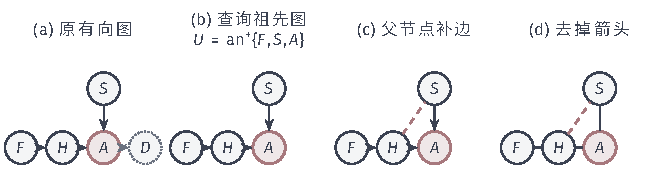
\includegraphics[width=156.951mm]{figures/06-probabilistic-graphical-models/01-representation/tikz/pgm-representations-ancestral-moralization/figure.pdf}
  \caption{报警查询的祖先道德图构造。原图以点线表示后代$D$及边$A\to D$。检验$F\perp S\mid A$时，祖先闭包为$U=\{F,H,A,S\}$，因此先去掉$D$及这条边。随后将$A$的父节点$H,S$相连，虚线表示新增的$H-S$边；再去掉原箭头，得到祖先道德图。红色的$A$是给定节点，检测分离时将其删除。}
  \label{fig:pgm-representations-ancestral-moralization}
\end{figure*}

图~\ref{fig:pgm-representations-ancestral-moralization}依次展示原有向图、查询祖先图、父节点补边和去箭头。点线标出随后筛除的后代，$H-S$虚线记录报警因子涉及的两个父节点。删除条件节点$A$后，路径$F-H-S$仍然连接，因此图不能推出$F\perp S\mid A$。若查询不包含$A$及其后代，祖先集合及由它产生的补边都可能不同。

\subsection{弦化与完美消元序}
\label{sec:pgm-representations-chordal-conversion}

推断时常常要逐个消去变量：第~\ref{chap:pgm-elimination}章会看到，消去$x_i$的标准做法是先把所有涉及$x_i$的局部因子相乘，再对$x_i$的各个状态求和。相乘后的新因子通常同时依赖$x_i$的若干个尚未删除的邻居；要让这个新作用域在无向图上仍是一个合法的团，这些邻居之间最好本来就有边。若它们缺边，就临时补一条边把作用域记录下来，这条边称为填充边；它也为无向表示改写成有向表示提供所需邻域结构。

图中不再有长度至少为四的诱导环时，就得到弦图。
给定节点顺序，本章将剩余邻域记为$N_k^+=\{v_\ell:\ell>k,\{v_k,v_\ell\}\in E\}$。
每个$N_k^+$中的剩余邻居都两两相连时，该顺序称为完美消元序；消元沿此顺序无需补边，边沿反序定向后，各节点的父节点也两两相连，形成完美有向图。

有限无向图存在完美消元序，当且仅当它是弦图。图~\ref{fig:pgm-representations-chordal-conversion}为四环加入$1-3$后，可按$(4,2,1,3)$消元：删除$4$或$2$时，剩余邻居$1,3$已由填充边相连；再删除$1$与$3$时，至多剩一个邻居，邻居两两相连的条件自动满足。将每条边从序中较晚的节点指向较早的节点，就得到无环且父集成团的有向图。定向采用消元次序的反序，因为当前节点的父节点正是尚未消去的邻居。

\begin{figure}[htbp]
  \centering
  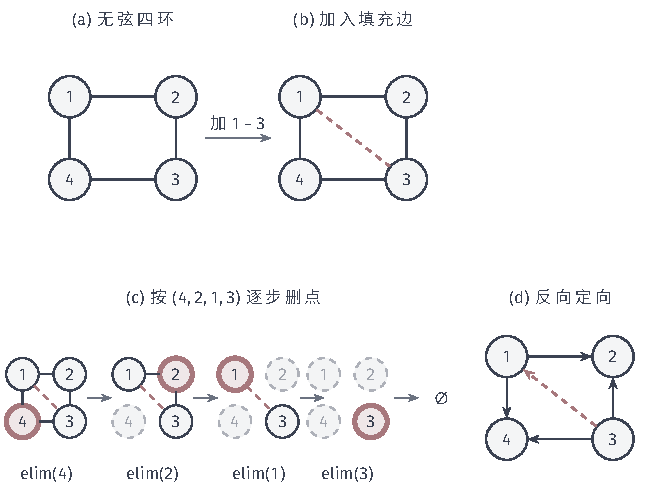
\includegraphics[width=112.000mm]{figures/06-probabilistic-graphical-models/01-representation/tikz/pgm-representations-chordal-conversion/figure.pdf}
  \caption{四环弦化及反序定向。加入虚线边$1-3$后，按完美消元序$(4,2,1,3)$删点；红色双圈为当前节点，灰色虚线轮廓为已删节点。各步下方的$\operatorname{elim}$标签记录被删除的节点，每一步的剩余邻居都两两相连。最后从序中较晚节点指向较早节点，实线箭头对应原四环的边，虚线箭头对应填充边。}
  \label{fig:pgm-representations-chordal-conversion}
\end{figure}

\Needspace{6\baselineskip}
\section{有向图与无向图的条件独立性关系}
\label{sec:pgm-representations-independence}

比较转换前后的独立性，需要精确描述两个集合：一个具体分布$p$实际满足的条件独立关系，以及一张图$\mathcal{G}$通过分离规则声明的条件独立关系。前者可能包含特殊参数造成的独立，后者则是结构对整类分布的保证。转换前后比较的，正是这两个集合之间的包含方向。下面先把它们写成集合，再定义三种刻画图与分布吻合程度的映射。

\subsection{独立性映射}
\label{sec:pgm-representations-maps}

将分布$p$的所有条件独立关系记为$\mathcal{I}(p)$：
\begin{equation}
  \mathcal{I}(p)
  =
  \bigl\{(A,B\mid S):
  \bm{X}_A\perp\bm{X}_B\mid\bm{X}_S\bigr\},
  \label{eq:pgm-representations-distribution-independences}
\end{equation}
查询集合$A,B,S\subseteq V$两两不交，$A,B$非空，条件集$S$允许为空。图的规则所蕴含的同类查询组成$\mathcal{I}(\mathcal{G})$：有向图按d-分离确定，无向图按无向分离确定。每项独立性按条件变量的分布成立；只在某个特殊条件值下成立的等式，未必属于这个集合。

这两个集合的包含方向决定图与分布的关系。图声明的独立越少，越不容易把本该相关的变量误判为独立；图声明的独立越多，对分布独立结构的限制越强。若图声明的关系全都属于分布的真实独立性，则称图为\term{独立性映射}（independency map, I-map）：图给出的每条独立保证都在分布中成立，但图可以只表达部分真实关系。若分布的全部独立性都能从图上读出，则称图为\term{依赖性映射}（dependency map, D-map）：图没有遗漏分布的任何独立，图上未被分离的变量在分布中也不独立。两个集合相等时，两项要求同时成立，图恰好刻画分布的全部独立结构，称为\term{完美映射}（perfect map）。

\begin{definition}[三类独立性映射]
  \label{def:pgm-representations-maps}
  对同一组随机变量的分布$p$与图$\mathcal{G}$，有
  \begin{equation}
    \begin{aligned}
      \mathcal{G}\text{是}p\text{的I-map}
      &\iff \mathcal{I}(\mathcal{G})\subseteq\mathcal{I}(p),\\
      \mathcal{G}\text{是}p\text{的D-map}
      &\iff \mathcal{I}(p)\subseteq\mathcal{I}(\mathcal{G}),\\
      \mathcal{G}\text{是}p\text{的完美映射}
      &\iff \mathcal{I}(\mathcal{G})=\mathcal{I}(p).
    \end{aligned}
    \label{eq:pgm-representations-map-inclusions}
  \end{equation}
\end{definition}

有向模型的可靠性保证$\mathcal{G}$是$p$的I-map；忠实性的反向蕴含再要求D-map方向成立，使有向图$\mathcal{G}$成为$p$的完美映射。这里的忠实性要求分布中的条件独立都能由图的d-分离解释，它用于排除特殊参数产生的额外独立性；其在关系识别中的作用可参考\BookChapterRef{chap:causal-inference}{卷2《数学准备：概率、因果与决策》中“因果响应”章}。

完全无向图与无边图提供了两个包含关系的极端。完全图没有分离任何两个非空节点集，因此没有独立性声明，对任意$p$都是I-map。无边图则声明所有互不相交的变量组在给定其他不交变量后独立，它的声明集包含任意$p$的真实关系，故总是D-map，通常却不是$p$的I-map。D-map的“依赖”可从逆否关系理解：对给定的$A,B,S$，图没有用$S$分离$A,B$时，$\bm{X}_A$与$\bm{X}_B$在$p$中给定$\bm{X}_S$也不独立。该保证覆盖全部查询。建模通常先满足I-map要求，因为任何错误的独立性约束都会将目标分布$p$排除在模型类之外\scite{pgm-koller2009}。

任何完全图都是I-map，但它一条独立都不声明，作为模型过于臃肿。建模时通常在保证I-map（不产生错误独立）的前提下尽量删边，因为边越少、因子越小、推断越省。若一张I-map的任一边被删后都会产生分布并不满足的错误声明，就称为\term{最小I-map}（minimal I-map）：再删任何一条边都会破坏安全性。这种最小性只针对当前图的单边删除，既不决定全体候选图中的最少边数，也不决定唯一图。例如两个二元变量取
\[
  p(0,0)=p(1,1)=0.4,\qquad
  p(0,1)=p(1,0)=0.1.
\]
两边缘都满足$p(X_1=0)=p(X_2=0)=0.5$，但$p(0,0)\ne0.25$，所以两变量依赖。$X_1\to X_2$与$X_1\leftarrow X_2$都没有额外独立声明；删边则会要求两变量独立，因此两图都是最小I-map。由此可见，单边删除的最小性保留了依赖，却无法确定方向。在一般图中，这种最小性还可能与遗漏其他真实独立性同时出现。

比较两张图时也可用同一包含方向：若$\mathcal{I}(\mathcal{G}_2)\subseteq\mathcal{I}(\mathcal{G}_1)$，称$\mathcal{G}_2$为$\mathcal{G}_1$的I-map。$\mathcal{G}_2$的独立性约束较少，仅受这些Markov约束、没有额外参数限制的分布族就较大。道德化与添加填充边通常给出这类较弱的独立性描述。

\subsection{d-分离的无向判据}
\label{sec:pgm-representations-ancestral-moralization}

第~\ref{sec:pgm-representations-ancestral-graphs}节构造的祖先道德图不只是示意，它恰好给出一个可操作的判据：d-分离不必再逐条路径分辨碰撞点，而可以完全转成无向图上的“删节点看连通”。选取查询祖先后，保留节点中的每个条件因子都只涉及这些节点；道德化再将其共同父节点相连。对所得无向图检查分离，可以精确回答原有向图的d-分离查询。

对有限DAG中两两不交的$A,B,S$，其中$A,B$非空，先取$U=\operatorname{an}^{+}(A\cup B\cup S)$，再在诱导图$\mathcal G[U]$上道德化。此时删去$S$后的无向分离，与原图中给定$S$的d-分离等价。这个等价关系只涉及图；后文将结合函数分解，证明分离查询所要求的概率独立性。

该判据在图上成立，因而与条件表参数及分布正性无关。检测按祖先闭包、诱导子图、道德化、删除条件节点$S$的次序进行：一个已观测的碰撞点在最后一步被删去，它的两个父节点之间的补边却应保留。先删除碰撞点会漏掉这条边，改变查询结果。Lauritzen的教材系统讨论祖先道德图与全局Markov性质\scite{pgm-lauritzen1996}。

对图~\ref{fig:pgm-representations-ancestral-moralization}中的$F\perp S\mid A$查询，最后删去$A$后，新增的$H-S$边仍留下路径$F-H-S$，所以当前图没有条件独立的保证。检验$F\perp S$时，祖先集合只有$\{F,S\}$，其余$H,A,D$都被去掉，剩余无边图给出独立性。同一原图的两个查询因此使用不同的祖先图，补边随$(A,B\mid S)$变化；未分离的查询仍可能在特殊参数下独立。

祖先闭包既保留端点，也保留导致间接联系的节点。例如$X_1\leftarrow X_0\to X_2$中，查询$X_1\perp X_2$需要$X_0$这个共同祖先；若仅留下$\{1,2\}$，两节点之间的联系会被误删。观测节点的祖先也有作用：在$X_1\to X_3\leftarrow X_2$、$X_3\to X_4$中，给定$X_4$激活了$X_3$处的碰撞点。查询$\{1\}$与$\{2\}$给定$\{4\}$时，祖先图保留$X_3$，随后道德化生成$1-2$边，记录这条被激活的联系。

若改为一次性道德化整个报警模型，新增边在所有查询中都保留。即使没有给定$A$，路径$F-H-S$也存在，原来的$F\perp S$就无法从整张道德图读出。\emph{整个有向图的道德图}用于重组联合函数的全部作用域，\emph{为查询构造的祖先道德图}则用于精确回答某项分离；整体图通常声明的独立性更少，其关系为
\begin{equation}
  \mathcal{I}\bigl(\operatorname{mor}(\mathcal{G})\bigr)
  \subseteq \mathcal{I}(\mathcal{G}),
  \label{eq:pgm-representations-moral-inclusion}
\end{equation}
整体图中被$S$分离的两侧，在较小的查询祖先道德图中仍被分离，所以整体图能证明部分d-分离。整体图中连通时，查询祖先图却可能已删除造成连通的节点或补边，因此原有向图仍可能满足这项d-分离。

\subsection{有向图独立性结论的证明}
\label{sec:pgm-representations-directed-proofs}

本节集中补全第~\ref{chap:pgm-directed}章引用但未展开的几个证明，第一次阅读时若主要关心结论与转换方法，也可以先跳过本节、直接进入第~\ref{sec:pgm-representations-factorizations}节的因子分解比较。证明的主线是：先用祖先道德图让局部因子的作用域全部落成团，从而把第~\ref{chap:pgm-undirected}章“分离后两侧分别归一化”的技巧搬到有向图上；再据此依次证明d-分离的可靠性、有向Markov毯以及模型类完备性。下面先说明局部条件分布如何归一化并产生联合分解，作为后续证明的共同基础。

\begin{proof}[引理~\ref{lem:pgm-directed-normalization}的证明]
取拓扑序中最后的节点，它没有子节点，只出现在自己的局部条件因子内。对其取值关于$\mu_i$积分，该因子由局部归一化变成$1$。继续逆拓扑序消去剩余节点，非负性允许用Tonelli定理交换积分次序，最后整个乘积的积分为$1$。有限离散状态下，同一操作就是逐节点求和。

求祖先集合的边缘分布时，仅需消去$V\setminus W$。集合$W$包含各节点的全部祖先，故$V\setminus W$中的节点没有位于$W$的子节点。逆拓扑序处理补集时，当前节点在补集中的子节点也已被消去，所以它仍只出现在自己的因子中。每次积分都将此因子变为一，最终留下式~\eqref{eq:pgm-directed-ancestral-marginal}中祖先节点的因子。
\end{proof}

\begin{proof}[定理~\ref{thm:pgm-directed-ordered-factor}的证明]
使用有序Markov假设指定的拓扑序，将联合概率按链式法则展开：
\[
  p(x_1,\ldots,x_d)=
  \prod_{i=1}^{d}p(x_i\mid x_1,\ldots,x_{i-1}).
\]
父节点都在当前节点之前。式~\eqref{eq:pgm-directed-ordered}使每个节点的条件分布只需保留前驱中的父节点变量：
\[
  p(x_i\mid\bm{x}_{\operatorname{pre}(i)})
    =p(x_i\mid\bm{x}_{\operatorname{pa}(i)}).
\]
代回链式法则，就得到式~\eqref{eq:pgm-directed-factorization}的父子分解。条件等式按前驱配置的分布几乎处处成立，因此还需说明零概率配置不会破坏乘积相等。

在有限离散情形，将按父配置选定的条件表记为$q_i$。父配置具有正概率时，$q_i$就是原分布的相应条件概率；父配置概率为零时，才可任选一行归一化概率来补全。完整前驱配置为零，未必意味着它包含的父配置也为零，所以不能据此前缀任意改变一行已经确定的父条件表。链式条件分布在零概率前驱上的版本可任意选择，与父条件表的补全范围需要分开。

记原分布前$k$个变量的边缘质量函数为$p_k$，并定义局部乘积
\[
  \widehat p_k(x_1,\ldots,x_k)
    =\prod_{i=1}^k q_i(x_i\mid\bm{x}_{\operatorname{pa}(i)}),
  \qquad \widehat p_0=p_0=1.
\]
我们按前缀长度证明$\widehat p_k=p_k$。若某个前缀满足$p_k(x_1,\ldots,x_k)>0$，下一节点的父配置也有正概率。有序Markov性质便将该前缀下的链式条件概率约简为已选定的$q_{k+1}$，因而
\[
  \begin{aligned}
    \widehat p_{k+1}
      &=\widehat p_k\,q_{k+1}
       =p_k\,p(x_{k+1}\mid x_1,\ldots,x_k)\\
      &=p_{k+1}.
  \end{aligned}
\]
若旧前缀的概率为零，归纳假设给出$\widehat p_k=0$，乘上下一张合法条件表后仍为零；原分布中任一延长前缀的概率也不超过旧前缀概率，所以$p_{k+1}=0$。这一步不改变正概率父配置上的条件表，也允许在零概率父配置上采用先前任意补全的行。两种情况覆盖全部前缀，从而在$k=d$得到所需联合分解。

连续密度则使用相应条件版本和积分的链式法则，得到几乎处处相同的联合密度。某个点的密度为零并不等同于离散前缀事件的概率为零，所以上面的逐配置归纳只用于有限离散情形。这一展开及约简都沿最初指定的同一拓扑序进行。
\end{proof}

\begin{proof}[定理~\ref{thm:pgm-directed-factor-local}的证明]
固定节点$i$，取非后代集合$N=\operatorname{nd}(i)$。其中各节点的祖先都仍在$N$中：若祖先是$i$或其后代，该节点就会成为$i$的后代；而$i$本身的祖先也在$N$内。因此，$N$与$N\cup\{i\}$都是祖先闭合集合，可以用引理~\ref{lem:pgm-directed-normalization}边缘化：
\[
  \begin{aligned}
    p(x_i,\bm{x}_N)
      &=q_i(x_i\mid\bm{x}_{\operatorname{pa}(i)})
        \prod_{j\in N}q_j(x_j\mid\bm{x}_{\operatorname{pa}(j)})\\
      &=q_i(x_i\mid\bm{x}_{\operatorname{pa}(i)})p(\bm{x}_N).
  \end{aligned}
\]
在有效条件值上约去非后代的边缘分布，得到$p(x_i\mid\bm{x}_N)=q_i(x_i\mid\bm{x}_{\operatorname{pa}(i)})$。再消去$N\setminus\operatorname{pa}(i)$，可见$q_i$也给出$p(x_i\mid\bm{x}_{\operatorname{pa}(i)})$的一个版本。给定父节点后，其他非后代不再改变节点的条件分布，局部Markov性质因而成立。

任一固定拓扑序都满足$\operatorname{pre}(i)\subseteq N$。在刚得到的局部独立关系中消去其余非后代，就获得该顺序下的有序Markov性质。由此，一个父子分解先推出局部性质，再推出所有拓扑序的有序性质。
\end{proof}

全局证明将查询祖先图内的因子分为两组。下面以离散求和书写；连续变量具有联合密度时，使用相应基准测度的积分，非负性使Tonelli定理适用。

\begin{proof}[定理~\ref{thm:pgm-directed-soundness}的证明]
取$p\in\mathcal{M}(\mathcal{G})$，并设查询满足$A\perp_{\mathcal{G}}B\mid S$。定理~\ref{thm:pgm-directed-ordered-factor}将$p$写成$\mathcal{G}$上的条件因子乘积，以$q_i(x_i\mid\bm{x}_{\operatorname{pa}(i)})$记节点$i$的因子。取查询祖先集合$R=\operatorname{an}^{+}(A\cup B\cup S)$，由引理~\ref{lem:pgm-directed-normalization}消去$V\setminus R$，留下
\[
  p(\bm{x}_R)=
  \prod_{i\in R}q_i(x_i\mid\bm{x}_{\operatorname{pa}(i)}).
\]
每个因子的作用域$\{i\}\cup\operatorname{pa}(i)$都在$\operatorname{mor}(\mathcal{G}[R])$中构成团。因此，删去$S$后，同一个因子剩余的节点都在同一连通分量中；两两相连的节点无法分属不同分量。

在$\operatorname{mor}(\mathcal{G}[R])\setminus S$中，将与$A$相交的分量合为$C$，其他节点合为$D=R\setminus(C\cup S)$。祖先道德化判据保证$B\subseteq D$。将涉及$C$的因子相乘记为$g(\bm{x}_C,\bm{x}_S)$，涉及$D$的因子相乘记为$h(\bm{x}_D,\bm{x}_S)$，其余只涉及$S$的因子相乘记为$k(\bm{x}_S)$，得到
\[
  p(\bm{x}_R)=
  g(\bm{x}_C,\bm{x}_S)
  h(\bm{x}_D,\bm{x}_S)
  k(\bm{x}_S).
\]
将未查询的$C\setminus A$和$D\setminus B$变量分别从两侧消去，所得函数记为$g_A,h_B$。乘积因此仍分为查询的两侧：
\[
  p(\bm{x}_A,\bm{x}_B,\bm{x}_S)=
  g_A(\bm{x}_A,\bm{x}_S)
  h_B(\bm{x}_B,\bm{x}_S)
  k(\bm{x}_S).
\]
固定具有正且有限边缘质量或密度的$\bm{x}_S$，将两侧总权重分别记为$G(\bm{x}_S)=\sum_{\bm{x}_A}g_A(\bm{x}_A,\bm{x}_S)$和$H(\bm{x}_S)=\sum_{\bm{x}_B}h_B(\bm{x}_B,\bm{x}_S)$。归一化条件联合分布时，这两个常数各自归一化一侧函数：
\[
  \begin{aligned}
    p(\bm{x}_A,\bm{x}_B\mid\bm{x}_S)
      &=\frac{g_A(\bm{x}_A,\bm{x}_S)}{G(\bm{x}_S)}
        \frac{h_B(\bm{x}_B,\bm{x}_S)}{H(\bm{x}_S)}\\
      &=p(\bm{x}_A\mid\bm{x}_S)
        p(\bm{x}_B\mid\bm{x}_S).
  \end{aligned}
\]
上述比值使用正概率条件事件或几乎处处的有效条件密度。两侧条件边缘相乘，便得到目标条件独立性。函数可以在部分联合配置取零，这个证明仍然成立。
\end{proof}

\begin{proof}[定理~\ref{thm:pgm-directed-markov-blanket}的证明]
以$O=V\setminus(\{i\}\cup\operatorname{mb}(i))$表示毯外节点。$O=\varnothing$时，独立侧为空，结论平凡成立。取$O\neq\varnothing$，考察从$i$到$O$中任一节点的路径。它的首步必经父节点或子节点，两类节点都在$\operatorname{mb}(i)$中。

首步经过父节点$j\to i$时，$j$在路径上有一个箭尾，是非碰撞点；它又满足$j\in\operatorname{mb}(i)$，所以被观测后阻断路径。首步经$i\to j$再沿$j\to k$离开时，子节点$j$同样是已观测的非碰撞点。若路径以$i\to j\leftarrow k$开始，$j$是已观测的碰撞点，但$k$是子节点的另一个父节点，也在$\operatorname{mb}(i)$内。此时$k$仍不是路径终点，且$k\to j$的箭尾使它成为已观测的非碰撞点，路径转而在这里被阻断。

三种首段覆盖了从$i$到$O$的所有路径，每条都被$\operatorname{mb}(i)$阻断，故$i\perp_{\mathcal G}O\mid\operatorname{mb}(i)$。应用定理~\ref{thm:pgm-directed-soundness}的可靠性，得到节点与毯外变量的条件独立。

在有效条件分布上，局部函数也给出同一屏蔽关系。按定理~\ref{thm:pgm-directed-ordered-factor}分解联合概率，给定其余变量后，只有节点$i$及其子节点的因子仍含$x_i$：
\begin{equation}
  \begin{aligned}
    p(x_i\mid\bm{x}_{V\setminus\{i\}})
      &\propto q_i(x_i\mid\bm{x}_{\operatorname{pa}(i)})\\
      &\quad{}\times
      \prod_{j\in\operatorname{ch}(i)}
        q_j(x_j\mid\bm{x}_{\operatorname{pa}(j)}).
  \end{aligned}
  \label{eq:pgm-directed-blanket-conditional}
\end{equation}
右侧的其他自变量全在$\operatorname{mb}(i)$中，因而对$x_i$归一化后，条件分布仍只使用毯内变量。这里的比例式用于条件分布有定义的配置；零概率条件配置采用第~\ref{chap:pgm-directed}章说明的条件分布版本。
\end{proof}

上述结果连起了第~\ref{chap:pgm-directed}章的四种表述：定理~\ref{thm:pgm-directed-ordered-factor}由有序Markov性质得到因子分解，定理~\ref{thm:pgm-directed-soundness}再由分解得到全局性质，引理~\ref{lem:pgm-representations-global-to-local}由全局得到局部，最后定理~\ref{thm:pgm-directed-factor-local}的边缘化论证由局部得到任一拓扑序的有序性质。于是式~\eqref{eq:pgm-directed-equivalence}的等价关系成立；各步都允许联合分布在某些配置取零。

可靠性只回答了“被d-分离的一定独立”，完备性还要回答相反的一面：没有被d-分离的查询，模型类中是否真的存在一个分布让两端相关？若不存在，d-分离规则就漏报了某些结构强制的独立。完备性证明通过构造“依赖见证”分布完成。最简单的连续情形只含一个碰撞点（或其后代被观测），可用高斯条件协方差直接算出非零依赖；一般图含多个碰撞点、多条路径时，不同路径的数值作用可能相互抵消，需要随后的非平凡性引理统一处理。对于图$X\to Z\leftarrow Y$及$Z\to D$，定义
\[
  \begin{aligned}
    X&=\varepsilon_X,& Y&=\varepsilon_Y,\\
    Z&=X+Y+\varepsilon_Z,& D&=Z+\varepsilon_D,
  \end{aligned}
\]
四个噪声相互独立，均取$\mathcal{N}(0,1)$分布。独立根节点使$X,Y$边缘独立，整个系统满足上述有向分解。噪声方差相加得到$\operatorname{Var}(Z)=3$，而$D=Z+\varepsilon_D$再增加一项独立噪声，所以$\operatorname{Var}(D)=4$。两个根变量与$Z$的协方差均为$1$；与$D$的协方差也均为$1$，因为新增噪声与根变量独立。观测碰撞点或其后代后，可用这些量和高斯条件协方差公式直接计算两根节点的关系：
\[
  \begin{aligned}
    \operatorname{Cov}(X,Y\mid Z)
      &=0-\frac{1\cdot1}{3}=-\frac13,\\
    \operatorname{Cov}(X,Y\mid D)
      &=0-\frac{1\cdot1}{4}=-\frac14.
  \end{aligned}
\]
条件协方差可由回归残差得到：分别将两个根变量对观测作线性回归，再计算残差的协方差。例如观测$Z$时，两个回归系数均为$1/3$，残差为$X-Z/3$与$Y-Z/3$，其协方差是$0-1/3-1/3+3/9=-1/3$；观测$D$时同理将系数换为$1/4$。联合高斯的残差与观测独立，因而该值就是条件协方差。上面两个非零结果分别给出观测碰撞点及其后代后的依赖；要覆盖一般有向图的所有活跃路径，还需要下一步的非平凡性结果。

一般图的活跃路径可含多个碰撞点，通向条件节点的路径也可能交会。不同路径的数值作用可能抵消，因此非零边系数本身不足以提供依赖见证。图~\ref{fig:pgm-directed-cancellation}展示一个明确的抵消参数：
\[
  X=\varepsilon_X,\qquad
  Z=X+\varepsilon_Z,\qquad
  Y=-X+Z+\varepsilon_Y,
\]
噪声仍相互独立且服从$\mathcal N(0,1)$。代入中间变量后得到$Y=\varepsilon_Z+\varepsilon_Y$，故$X\perp Y$：三个边系数虽然非零，直接与间接路径上的作用却恰好相消。若将$X\to Y$的系数改为$-1+\delta$，就有$\operatorname{Cov}(X,Y)=\delta$。当$\delta\ne0$时，这项额外独立性消失。

\begin{figure}[htbp]
  \centering
  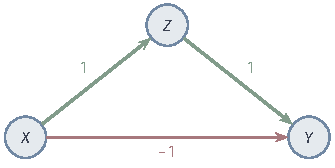
\includegraphics[width=56.653mm]{figures/06-probabilistic-graphical-models/01-representation/tikz/pgm-directed-cancellation/figure.pdf}
  \caption{直接与间接作用相消的高斯模型。$X\to Y$的系数为$-1$，经$Z$的两个系数均为$1$，代入后两项相消。两条路径对空条件集都活跃，这组参数却使$X$与$Y$独立。}
  \label{fig:pgm-directed-cancellation}
\end{figure}

完备性需要证明，对每项活跃查询，其条件独立约束并未在整个相容参数空间中恒成立。为检验这一点，先将条件独立写为一个等式，再将等式改写成模型参数的多项式取零。这样，图上的依赖见证问题就转成了参数空间中能否找到违反该等式的点。

高斯情形可以沿用刚才的条件协方差判据。记全体变量的协方差矩阵为$\bm\Sigma$；在非退化联合高斯模型中，两个标量条件独立，等价于它们的条件协方差为零。计算这个条件协方差需要对条件变量的协方差块$\bm\Sigma_{S,S}$求逆；乘以正的$\det(\bm\Sigma_{S,S})$后，可将逆矩阵带来的分母消去。所得量正是行指标为$(u,S)$、列指标为$(v,S)$的交叉子式，后面的分块行列式计算会给出这一关系。因此，这个子式取零等价于对应的标量条件协方差取零。

离散情形在$p(\bm x_S)>0$的配置上，将条件独立等式两侧的条件概率换成联合概率比值，再交叉相乘，得到下面的两项概率乘积之差。若$p(\bm x_S)=0$，相关联合质量也都为零，交乘式自动成立，无需在零概率事件上取比值。联合概率是有限个条件表项的乘积，边缘概率又是联合概率的有限和，所以该差也是条件表自由参数的多项式。

这里的“非零多项式”表示它不恒等于零，允许在特殊参数处取零；抵消例正是这样的特殊取值。下面的引理将活跃路径的图论条件转为多项式不恒为零的保证，之后的代数步骤由此选择一个违反独立约束的参数。离散结论及路径构造采用Meek的强完备性结果，高斯结论采用线性高斯有向图的多项式完备性结果\scite{pgm-directed-meek1995,pgm-koller2009}。

\begin{lemma}[条件独立约束的非平凡性]
  \label{lem:pgm-directed-nontrivial}
  设$\mathcal{G}=(V,E)$为有限有向无环图，$u,v\in V$为不同节点，$S\subseteq V\setminus\{u,v\}$，且$u,v$在$\mathcal{G}$中给定$S$时d-连接，则以下两项成立。
  \begin{enumerate}
    \item 对$i\in V$，在线性高斯系统
    \[
      X_i=\sum_{j\in\operatorname{pa}(i)}b_{i,j}X_j+\varepsilon_i,
      \qquad
      \varepsilon_1,\ldots,\varepsilon_d
      \mathrel{\overset{\mathrm{ind}}{\sim}}\mathcal N(0,1)
    \]
    中，记边系数为$\bm{\theta}$、协方差矩阵为$\bm{\Sigma}(\bm{\theta})$，则
    \[
      f_{u,v,S}(\bm{\theta})
      =\det\bm{\Sigma}_{(u,S),(v,S)}(\bm{\theta})
    \]
    是非零多项式。行指标按$u$及$S$排列，列指标按$v$及同一顺序的$S$排列；$S=\varnothing$时，该式为$\Sigma_{u,v}$。
    \item 固定每个节点至少含两个状态的有限状态空间，并用各行前$r_i-1$个概率参数化局部条件表。将联合概率与边缘概率写成这些参数的多项式后，在所有状态配置对应的条件独立多项式
    \[
      p(x_u,x_v,\bm{x}_S)p(\bm{x}_S)
      -p(x_u,\bm{x}_S)p(x_v,\bm{x}_S)
    \]
    中，至少有一个不是零多项式。
  \end{enumerate}
\end{lemma}

本章采用这一外部引理，下面的证明以它为前提。引理所处理的是活跃路径及碰撞点通向$S$的有向路径：从中提取保留连接的子图，并控制路径交会时的代数抵消。高斯模型可以使用任意正噪声方差，这里的单位方差子类已足够构造所需见证；逐坐标可逆缩放也保持条件独立性。具体地，若原噪声标准差为$\sigma_i>0$，令$Y_i=X_i/\sigma_i$，新噪声就具有单位方差，边系数则变为$b_{i,j}\sigma_j/\sigma_i$。这种缩放没有丢掉任何坐标信息，所以不会改变条件独立关系。

\begin{proof}[定理~\ref{thm:pgm-directed-completeness}的线性高斯部分]
集合$A,B$未被$S$ d-分离时，可选由活跃路径连接的$u\in A,v\in B$。将引理~\ref{lem:pgm-directed-nontrivial}的线性系统按拓扑序写为矩阵形式，得到$\bm X=\bm B\bm X+\bm\varepsilon$；系数矩阵$\bm{B}$严格下三角，非边元素为零。于是$\bm X=(\bm I-\bm B)^{-1}\bm\varepsilon$，再利用$\bm{B}^d=\bm 0$，得到
\[
  \begin{aligned}
    \bm{L}&=(\bm{I}-\bm{B})^{-1}
       =\bm{I}+\bm{B}+\cdots+\bm{B}^{d-1},\\
    \bm{\Sigma}(\bm{\theta})&=\bm{L}\bm{L}^{\top}.
  \end{aligned}
\]
有限矩阵和使协方差各元素都成为边系数的多项式；对任意实边系数，可逆的线性变换又保证$\bm{\Sigma}$正定。将条件协方差写入分块行列式，可得
\[
  f_{u,v,S}(\bm{\theta})
    =\det(\bm{\Sigma}_{S,S})
      \bigl(\Sigma_{u,v}
        -\bm{\Sigma}_{u,S}\bm{\Sigma}_{S,S}^{-1}
         \bm{\Sigma}_{S,v}\bigr).
\]
括号给出$\operatorname{Cov}(X_u,X_v\mid\bm X_S)$。$S$为空时，空矩阵行列式取$1$，矩阵求逆项无需执行。高斯条件分布的两个标量独立当且仅当这个协方差为零。引理保证$f_{u,v,S}$为非零多项式，所以可以选取使条件协方差非零的系数。

存在性还可落实为有限终止的枚举：逐渐增大有理数分子绝对值及正分母的上界，枚举有理边系数向量，用有理数运算计算行列式，找到非零值即停止。非零多项式在某个实参数点附近仍非零，有理向量的稠密性保证枚举能进入这个邻域。输出系数与单位独立高斯噪声定义了$\mathcal{M}_{\mathrm{LG}}(\mathcal{G})$中的分布，满足$X_u\not\perp X_v\mid\bm X_S$。若向量$\bm X_A,\bm X_B$条件独立，每对分量也应条件独立，因而与上述结果矛盾。这给出了查询的见证构造，但并未给出高效寻找见证的算法。
\end{proof}

有限离散模型改用条件表参数。每一行取前若干状态概率为自由参数，末状态概率由行和为$1$确定。各自由坐标大于$0$且每行自由坐标之和小于$1$，恰好保证整行严格为正。这些都是严格不等式，多行参数的笛卡尔积因而在有限维参数空间中形成开集；每行均匀分布给出其中一个点，说明该开集非空。联合概率与边缘概率都是这些参数的多项式。严格正性保证$p(\bm x_S)>0$，所以给定$S$时$X_u$与$X_v$条件独立，等价于每种状态配置都满足
\[
  \begin{aligned}
    &p(x_u,x_v,\bm x_S)p(\bm x_S)\\
    &\qquad{}-p(x_u,\bm x_S)p(x_v,\bm x_S)=0.
  \end{aligned}
\]

要从不恒为零走到这个严格正参数域内的见证，还需知道：非零多项式的零点不可能占满一个非空开集。下面用零点集的测度说明这一事实，也为随后同时避开多项额外独立约束作准备。

\begin{lemma}[非零多项式的零点集]
  \label{lem:pgm-representations-polynomial-zero-set}
  设$f$是$\mathbb R^m$上不恒为零的实多项式，$m\geq1$。其零点集具有$m$维Lebesgue测度零，因此不能包含非空开集。
\end{lemma}

\begin{proof}
记$\lambda_m$为$m$维Lebesgue测度。$m=1$时，非零多项式只有有限个实根，故零点集的测度为零。设结论对$m-1$个变量成立，将$m$元多项式按最后一个坐标$t$展开为
\[
  f(\bm y,t)=\sum_{\ell=0}^{K}a_\ell(\bm y)t^\ell,
  \qquad \bm y\in\mathbb R^{m-1}.
\]
至少有一个系数多项式$a_{\ell_0}$不恒为零。使所有系数同时为零的底点集合记为$E$，它包含在$a_{\ell_0}$的零点集中，因归纳假设而有$\lambda_{m-1}(E)=0$。在$E$之外，每个固定$\bm y$对应一元非零多项式，它的零点只有有限个，故沿$t$方向的截面测度为零。

先将零点集限制在盒$[-M,M]^m$内，其中$M$为正整数。在坏底点$E$上，截面长度至多为$2M$；在其余底点上，截面长度为零。零点集是闭集，可以对其非负指标函数使用Tonelli定理，按底点与最后一个坐标分别积分。积分只可能在零测的$E$上贡献至多$2M$，所以整个盒内零点集的$m$维测度仍为零。再令$M=1,2,\ldots$，这些盒覆盖全空间，可数个零测集的并仍为零测集。任一非空开集含有边长为正的小盒，具有正测度，因此不能包含在该零点集中。
\end{proof}

\begin{proof}[定理~\ref{thm:pgm-directed-completeness}的有限离散部分]
取活跃路径连接的$u\in A,v\in B$。引理~\ref{lem:pgm-directed-nontrivial}的第二项保证，有限组条件独立多项式中至少一项非零。由引理~\ref{lem:pgm-representations-polynomial-zero-set}，非零多项式在参数空间的非空开集上无法恒为零。严格正条件表参数域正是这样的开集，所以其中必有一点使选定多项式非零，至少一个独立等式随之失败。所得联合分布属于$\mathcal{M}_{\mathrm{disc}}^{+}(\mathcal{G})$，并满足$X_u\not\perp X_v\mid\bm X_S$。向量$\bm X_A\perp\bm X_B\mid\bm X_S$若成立，会推出所有坐标对条件独立，与选定坐标对的结论矛盾。故$\bm X_A\not\perp\bm X_B\mid\bm X_S$，有限离散类也存在所需见证。
\end{proof}

对固定有限图，所有节点对及条件集合的查询只有有限多组。为每项未分离查询选定一个非零检验多项式：高斯情形选上述交叉子式，离散情形选引理保证不恒为零的某一状态配置等式。该查询若出现额外独立性，选定多项式就必须取零。因此，导致该查询额外独立的坏参数集包含在一个零测集中，而不要求它恰好等于整个零点集。有限个这样的零点集之并仍为零测集，无法覆盖具有非空内部的合法参数域。选取并集之外的同一组参数，就能同时避免所有节点对查询的额外独立性；任何未分离的向量查询又含有一对活跃连接的坐标，故也不可能额外独立。

这一论证也覆盖正噪声方差自由变化的线性高斯模型，而不限于构造见证所用的单位方差子类。令$\tau_i>0$为第$i$项噪声方差，协方差变为$\bm\Sigma=\bm L\operatorname{diag}(\tau_1,\ldots,\tau_d)\bm L^\top$，其元素仍是边系数和方差坐标的多项式。每个检验多项式在所有$\tau_i=1$的子类中已不恒为零，所以在更大的参数空间中也不恒为零；正方差条件给出的域仍是非空开集。截距只改变均值，不影响这些条件独立判据，把截距也列作自由坐标后仍可使用同一零点集结论。因此，在上述没有额外约束的离散或线性高斯参数族中，忠实分布存在，不忠实参数组成零测集。真实系统可能具有特殊参数；接近抵消集合时，依赖还可能很弱，使有限样本难以分辨。

\subsection{两类独立性表示的差异}
\label{sec:pgm-representations-independence-differences}

查询祖先道德图随端点和条件集合而变化；一张固定的无向图未必能同时复现所有d-分离。例如碰撞结构$X_1\to X_3\leftarrow X_2$声明$X_1\perp X_2$，没有声明$X_1\perp X_2\mid X_3$。无向图若使$1$与$2$被空集分离，两节点之间原本就无路径；再删$3$仍然分离。这个单调性与碰撞查询的变化冲突，所以同一节点集合上无法找到完全相同的无向分离集合。特殊参数产生的分布仍可由两类图共同表示，当前反例比较的是图的全部独立性声明。

从无向图转向有向图也存在表达边界。图~\ref{fig:pgm-representations-chordal-conversion}左侧四环$1-2-3-4-1$没有对角边$1-3$或$2-4$，同时声明
\begin{equation}
  X_1\perp X_3\mid(X_2,X_4),\qquad
  X_2\perp X_4\mid(X_1,X_3).
  \label{eq:pgm-representations-cycle-independences}
\end{equation}
给这个骨架作无环定向，至少一个节点会同时接收两条环边。例如$2\to1\leftarrow4$的两父节点$2$与$4$不相邻，形成未遮蔽碰撞点。给定$\{1,3\}$会打开路径$2\to1\leftarrow4$，所以d-分离无法得到式~\eqref{eq:pgm-representations-cycle-independences}的第二项。

这一碰撞点可由拓扑序直接找出：四环中排在最后的节点，其两个邻居都在前，故两条边都指向它。更换拓扑序会改变碰撞的位置，仍会留下一个未遮蔽碰撞点。

改变骨架也无法保留原来的全部独立性。对有向图中两个不相邻节点$i,j$，无环性保证可以选一个节点，例如$i$，使$j$是它的非后代。$j$又不是$i$的父节点，第~\ref{chap:pgm-directed}章证明局部Markov性质时所用的图分离关系便给出$i\perp_{\mathcal G}j\mid\operatorname{pa}(i)$。这一步只涉及图；再应用可靠性，才得到相容分布中的$X_i\perp X_j\mid\bm{X}_{\operatorname{pa}(i)}$。无向图中的非邻接对则被其余全部节点分离。相邻对在两类图中都保留长度为一的路径，任何不含端点的条件集都无法阻断它。由此，全部图分离关系能确定邻接关系，两张图独立性集合相同时也必有同一骨架。

碰撞结构的观测激活与四环的两项对角条件独立，分别超出了另一类图在同一节点集上的完美表示范围，所以两类图的独立性表达能力一般互不包含。第~\ref{sec:pgm-representations-chordal-conversion}节的弦图和完美有向图则提供了可相互保留全部分离关系的结构条件。

\subsection{完美表示的条件}
\label{sec:pgm-representations-perfect-dags}

碰撞结构和无弦四环说明两类图的独立性表达能力一般互不包含。能够无损保留全部分离关系的结构由弦图以及“父集成团”的有向图给出，二者是同一性质在两种图上的体现。以下两个判定分别用于无向到有向、有向到无向的完美表示。

对于有限无向图，要在同一节点集合上用DAG保留全部分离关系，原图必须是弦图，而弦图也允许这种改写。选取一个完美消元序，将每条边从序中较晚的节点指向较早的节点，便得到所需的完美有向图。此时原剩余邻域成为父集，每个父集中的节点两两相连。


对有限DAG，同一节点集合上的完美无向表示，要求各节点父集内的节点两两相连；这个条件也足以保证表示存在。每个父集内的节点已经两两相连时，道德化无需额外补父节点之间的边，去掉方向后的骨架就是弦图，并保留同样的分离关系。

“完美有向图”的判定只用父集是否成团；“$\mathcal{D}$是$p$的完美映射”则比较图与某个分布的独立性。即使$\mathcal{D}$和$\mathcal{U}$的分离集合完全相等，特殊参数仍可能让$p$具有额外独立性。这两种转换保证的是图之间的完美表示，具体分布的完美映射还需忠实性。

原图不满足弦性时，可以添加边后再定向。图~\ref{fig:pgm-representations-chordal-conversion}为四环补$1-3$，产生极大团$\{1,2,3\}$与$\{1,3,4\}$。以$\mathcal{U}$记原图、$\widetilde{\mathcal{U}}$记弦化图，则有
\[
  \mathcal{I}(\widetilde{\mathcal{U}})
  \subseteq \mathcal{I}(\mathcal{U}).
\]
填充边增加可用路径，因而新分离集合只能缩小。四环的$X_2\perp X_4\mid(X_1,X_3)$仍能从新图读出，$X_1\perp X_3\mid(X_2,X_4)$却因为新增对角边而失去图上的保证。弦化换来了所需的消元和定向结构，也可能减少可见的独立性。

\section{有向图与无向图的因子分解关系}
\label{sec:pgm-representations-factorizations}

前两节从结构和独立性两个层面比较了两种图，本节转向第三个层面：局部函数怎样重组，才能在换图的同时保持联合分布的每一个概率值都不变。以下固定一个给定分布$p$，说明它的条件分布与团势如何互相改写，同时区分“对这一个分布的精确改写”与“转换后那张图所允许的整类自由参数模型”。后者通常比原来的分布族更大，因为一旦不再约束新表项之间的关系，模型就能表达转换前没有的分布。两种分解在归一化方式上的差异，决定了转换时必须额外处理的内容。

\subsection{两类因子分解的差异}
\label{sec:pgm-representations-normalization}

有向图把联合分布写成每个节点给定父节点的条件分布乘积：
\begin{equation}
  p(\bm{x})=\prod_{i\in V}
  p(x_i\mid\bm{x}_{\operatorname{pa}(i)}).
  \label{eq:pgm-representations-directed-product}
\end{equation}
每个父配置下，局部条件表都满足$\sum_{x_i}p(x_i\mid\bm{x}_{\operatorname{pa}(i)})=1$。从没有子节点的节点开始求和，它只在自己的条件因子中出现，这个因子因此变成$1$。剩余图仍无环，可以继续同样的操作，最后得到$\sum_{\bm{x}}p(\bm{x})=1$。局部归一化与无环结构共同保证了联合归一化。

Markov网络使用团上的非负势，另以全局配分函数归一化：
\begin{equation}
  p(\bm{x})=\frac{1}{Z}
  \prod_{C\in\mathcal{C}}\psi_C(\bm{x}_C),
  \qquad
  Z=\sum_{\bm{x}}\prod_{C\in\mathcal{C}}\psi_C(\bm{x}_C),
  \label{eq:pgm-representations-undirected-product}
\end{equation}
所选团作用域组成$\mathcal{C}$，其中可含极大团或较小团，且需满足$0<Z<\infty$。势表给出相对权重，对单个变量的求和可以异于$1$。不同势共享坐标，逐表归一化后，整体乘积仍需自己的归一化常数。将一个势乘以正常数时，$Z$同比缩放，分布$p$保持原样；这种尺度自由度构成势参数的冗余。

连续变量改用指定乘积测度的积分，函数需可测、非负且可归一化，局部密度也以积分为一理解。已给定非负团分解时，全局Markov性质允许零配置；从独立性反推团分解，则采用上一章说明的严格正性等条件。下面的条件表重组使用有限离散严格正分布，使每步条件归一化的分母都为正。

\subsection{从有向因子分解到无向因子分解}
\label{sec:pgm-representations-directed-to-undirected}

从有向因子分解转换到无向因子分解更直接。有向条件因子$p(x_i\mid\bm{x}_{\operatorname{pa}(i)})$虽然带有“$i$条件于父节点”的方向含义，但作为普通多变量函数，它只依赖$\{i\}\cup\operatorname{pa}(i)$这一组变量，见式~\eqref{eq:pgm-representations-directed-product}。只要在无向图中把这个“家庭集合”连成一个团，就可以直接把整张条件表当成该团上的势，函数值保持不变。整体道德化恰好完成补边，使每个家庭集合都成为团，因此原条件分布可作为该团的势：
\[
  \psi_{\{i\}\cup\operatorname{pa}(i)}
  (x_i,\bm{x}_{\operatorname{pa}(i)})
  =
  p(x_i\mid\bm{x}_{\operatorname{pa}(i)}),
\]
全部势相乘仍是原来的条件分布乘积；相同作用域的因子可以保留，也可以合并。原联合分布已归一化，故此时$Z=1$。若只保留极大团势，就给每个因子选择一个包含它的极大团，在团内相乘；未接收因子的团用常数$1$。每个因子参与一次，联合函数因此不变。极大团按包含关系覆盖局部作用域，适合完成这种分配；仅选节点数最多的团，可能遗漏其他作用域。

将报警模型的四个条件或先验因子分配给两个极大团，就得到
\begin{equation}
  \begin{aligned}
    p(f,h,a,s)&=p(f)p(s)p(h\mid f)p(a\mid h,s)\\
    &=\psi_{\{F,H\}}(f,h)\,
      \psi_{\{H,A,S\}}(h,a,s),\\
    \psi_{\{F,H\}}(f,h)&=p(f)p(h\mid f),\\
    \psi_{\{H,A,S\}}(h,a,s)&=p(s)p(a\mid h,s).
  \end{aligned}
  \label{eq:pgm-representations-alarm-potentials}
\end{equation}
新增的$H-S$边让道德图容纳报警因子的三元作用域，也使图上无法读出$F\perp S$。原因子保留的分布仍有这项独立性，对$a,h$求和便可验证：
\[
  \sum_h\sum_a p(f)p(s)p(h\mid f)p(a\mid h,s)
  =p(f)p(s).
\]
两势中的条件归一化关系让该等式继续成立，而新图的路径规则没有编码这些关系。若把两势表作为自由权重任意修改，图所允许的其他分布就可能失去$F\perp S$。

用人工参数可计算报警观测后的关系变化。取$p(F=1)=0.1$、$p(S=1)=0.05$，以及$p(H=1\mid F=1)=0.8$、$p(H=1\mid F=0)=0.1$，得到$p(H=1)=0.17$。在$(h,s)=(0,0),(1,0),(0,1),(1,1)$四种配置下，令$p(A=1\mid h,s)$依次为$0.01,0.9,0.7,0.99$。这些值只用于演示模型计算。因$H$与$S$边缘独立，报警概率为
\[
  \begin{aligned}
    p(A=1)
    &=0.83\times0.95\times0.01
      +0.17\times0.95\times0.9\\
    &\quad+0.83\times0.05\times0.7
      +0.17\times0.05\times0.99\\
    &=0.1907.
  \end{aligned}
\]
观测到报警后，再给定不同的传感器状态，过热的后验概率分别为
\begin{equation}
  \begin{aligned}
    p(H=1\mid A=1,S=0)
    &=\frac{0.17\times0.9}
    {0.17\times0.9+0.83\times0.01}
    \approx0.9485,\\
    p(H=1\mid A=1,S=1)
    &=\frac{0.17\times0.99}
    {0.17\times0.99+0.83\times0.7}
    \approx0.2246.
  \end{aligned}
  \label{eq:pgm-representations-alarm-posteriors}
\end{equation}
两个后验概率不同，说明这组参数在给定碰撞点后产生了依赖。式~\eqref{eq:pgm-representations-alarm-potentials}的团势积与原有向积相同，因而得到同样的计算结果。$H-S$补边记录无向函数所需的作用域，分布中的概率关系在转换前后保持不变。

道德化让有$k$个父节点的子节点及其父节点组成$k+1$元团，父节点间至多增加$\binom{k}{2}$条边。每变量有$r$种状态时，稠密$(k+1)$元表包含$r^{k+1}$项。原来的一般条件表已使用同一家庭作用域，所以这张团表本身未必增加存储量。多个家庭叠加却可能形成更大的最大团；若将原小因子全部合成该团的一般表，就会增加需要保存的组合，并失去可利用的细分计算结构。

推断的主要开销由消元时形成的联合因子决定，输入边数只提供部分结构信息。道德图仍可能含无弦环，随后消元还需填充边。道德化完成的是原因子作用域的无向表示；寻找较低代价的消元结构，还要另外选择顺序。

\subsection{从无向因子分解到有向因子分解}
\label{sec:pgm-representations-undirected-to-directed}

反方向（从无向势恢复成一组有向条件表）更有讲究。最省事的做法是直接套用链式法则：沿任意顺序把联合分布写成每个变量给定全部前驱的条件分布乘积，但这样每个节点的父集几乎包含所有前驱，得到的是一张稠密有向图，完全丢掉了原无向图的稀疏邻接。若希望保留原邻接、让每个节点的父集只含它在消元时的剩余邻居，就必须借助弦图的完美消元序——这正是第~\ref{sec:pgm-representations-chordal-conversion}节引入弦化的原因。

具体做法是逐次消元，每消去一个变量就把它“当时涉及的全部因子”整理成一张以剩余邻居为条件的条件表。设$p$严格为正，在弦图$\mathcal{U}$上已有团分解，取完美消元序$v_1,\ldots,v_d$。逐次消元时，要保持如下作用域条件：处理$v_k$前，每个具有非空作用域的当前因子，都定义在剩余诱导图$\mathcal{U}[\{v_k,\ldots,v_d\}]$的团上；作用域为空的常数因子也保留在乘积中。初始因子满足此条件，所以第$1$步可用。

若第$k$步开始时条件成立，含$v_k$的团因子，其余坐标必是$v_k$尚未删除的邻居，属于$N_k^+$。相乘并消去$v_k$后，新的作用域仍包含在$N_k^+$中；该集合的节点在完美消元序下两两相连，所以非空的新作用域仍是下一张剩余图的团。若新作用域为空，就得到常数因子。不含$v_k$的因子保持原样，作用域条件由此逐步保持。

第$k$步将当前含$v_k$的因子收集为$\mathcal{B}_k$，相乘后只需$v_k$及$N_k^+$的取值。对$v_k$求和得到剩余邻居上的新因子，再用它归一化当前节点：
\begin{equation}
  \begin{aligned}
    b_k(x_{v_k},\bm{x}_{N_k^+})
    &=\prod_{\psi\in\mathcal{B}_k}\psi,\\
    a_k(\bm{x}_{N_k^+})
    &=\sum_{x_{v_k}}b_k(x_{v_k},\bm{x}_{N_k^+}),\\
    q_k(x_{v_k}\mid\bm{x}_{N_k^+})
    &=\frac{b_k(x_{v_k},\bm{x}_{N_k^+})}
    {a_k(\bm{x}_{N_k^+})}.
  \end{aligned}
  \label{eq:pgm-representations-bucket-normalization}
\end{equation}
函数可以实际忽略部分已列坐标。将$\mathcal{B}_k$的因子从当前乘积中移除，换入$a_k$，就将$v_k$边缘化了。当新因子有非空作用域时，它仍定义在团上，$a_k$所用的邻接关系都已存在于原弦图中。末步$N_d^+=\varnothing$，此时$a_d$是常数，无需给它指定一个非空团。

所得$q_k$还需与原联合分布的条件概率对应。消去$v_1,\ldots,v_{k-1}$后，当前乘积正比于剩余变量的联合边缘分布。给定其他剩余坐标时，$\mathcal{B}_k$之外的因子都不含$v_k$，在条件比值中可约掉。因而$q_k$正是该边缘分布中$v_k$给定所有剩余变量的条件分布，并且按式~\eqref{eq:pgm-representations-bucket-normalization}只依赖$N_k^+$。这个结果使用消元到当前步骤的全部相关因子，原来一张团势单独归一化通常不会给出同一条件表。

每步的归一化给出$b_k=q_k a_k$。将这些等式依次代回原势乘积，全部节点消去后留下的常数乘积等于$Z$，得到
\begin{equation}
  \begin{aligned}
    \prod_{C\in\mathcal{C}}\psi_C(\bm{x}_C)
    &=Z\prod_{k=1}^d q_k(x_{v_k}\mid\bm{x}_{N_k^+}),\\
    p(\bm{x})&=\prod_{k=1}^d q_k(x_{v_k}\mid\bm{x}_{N_k^+}).
  \end{aligned}
  \label{eq:pgm-representations-telescoping-product}
\end{equation}
以$N_k^+$为$v_k$的父集，便获得按完美消元序反向定向的有向图。父节点在消元时晚于当前节点，所以拓扑序是消元序的逆序。每张新条件表已归一化，而求出它们的过程包含了原分布的边缘化和全局归一化计算；这些工作随表重组一同完成\scite{pgm-koller2009}。

原图非弦时，剩余邻居可能缺边。消元通常产生同时依赖这些邻居的新因子，需要添加填充边容纳作用域；在填充后的弦图上仍可按上述方法精确转换。这个结构要求针对整类严格正团分布：同一构造要处理所有可能参数，就需要容纳相应的中间作用域。固定参数时，新因子还可能进一步分解，独立分布甚至无需这些联系，因此实际保留的边还可受函数结构影响。

对例~\ref{ex:pgm-undirected-cycle}的四节点环，可将每步消元与新条件表直接算出。四变量都取$\{0,1\}$，四条环边使用相同势：
\begin{equation}
  \psi_{\{i,j\}}(x_i,x_j)=
  \begin{cases}
    2,&x_i=x_j,\\
    1,&x_i\ne x_j.
  \end{cases}
  \label{eq:pgm-representations-cycle-potentials}
\end{equation}
先将四势相乘作为未归一化权重。按图~\ref{fig:pgm-representations-chordal-conversion}的顺序消去$4$，涉及它的两个边势产生
\begin{equation}
  \begin{aligned}
    m(x_1,x_3)
    &=\sum_{x_4}\psi_{\{1,4\}}(x_1,x_4)
    \psi_{\{3,4\}}(x_3,x_4)\\
    &=
    \begin{cases}
      5,&x_1=x_3,\\
      4,&x_1\ne x_3.
    \end{cases}
  \end{aligned}
  \label{eq:pgm-representations-cycle-message}
\end{equation}
在$x_1=x_3=0$时，求和的两项为$2\times2$与$1\times1$，合为$5$；两端不同时，各项为$2$，合为$4$。新函数$m$同时使用$1,3$，对应新增的$1-3$填充边。再消去$2$得到同样的$m(x_1,x_3)$，两函数相乘后的剩余权重为$m(x_1,x_3)^2$，故
\[
  Z=2\times5^2+2\times4^2=82.
\]

前两步的条件分布记为$q_4(x_4\mid x_1,x_3)$和$q_2(x_2\mid x_1,x_3)$，下标表示对应变量节点。各自的分子是两个关联边势的乘积，分母为$m$。当$x_1=x_3$，中间变量取同一状态的概率为$4/5$，另一状态为$1/5$；当$x_1\ne x_3$，两状态概率均为$1/2$。

消去$4$和$2$后，对剩余权重$m(x_1,x_3)^2$继续消去$1$。无论$x_3$取何值，都有
\[
  \sum_{x_1}m(x_1,x_3)^2=5^2+4^2=41,
\]
由此$q_1(x_1\mid x_3)=m(x_1,x_3)^2/41$。最后两个状态$x_3=0,1$各留下权重$41$，总和$Z=82$使$q_3(x_3)=41/82=1/2$。后两张条件表因此为
\begin{equation}
  q_3(x_3)=\frac12,\qquad
  q_1(x_1\mid x_3)=
  \begin{cases}
    25/41,&x_1=x_3,\\
    16/41,&x_1\ne x_3.
  \end{cases}
  \label{eq:pgm-representations-cycle-root-tables}
\end{equation}
根据各条件表的输入，父集分别是$\operatorname{pa}(3)=\varnothing$、$\operatorname{pa}(1)=\{3\}$及$\operatorname{pa}(2)=\operatorname{pa}(4)=\{1,3\}$，对应边$3\to1$、$1\to2$、$3\to2$、$1\to4$和$3\to4$。把四条件表相乘，两分母$m$与分子中的平方约去，得到原来的联合概率：
\[
  \begin{aligned}
    q_3q_1q_2q_4
    &=\frac12\,
      \frac{m(x_1,x_3)^2}{41}\,
      \frac{\psi_{\{1,2\}}\psi_{\{2,3\}}}{m(x_1,x_3)}\,
      \frac{\psi_{\{1,4\}}\psi_{\{3,4\}}}{m(x_1,x_3)}\\
    &=\frac{
      \psi_{\{1,2\}}\psi_{\{2,3\}}
      \psi_{\{1,4\}}\psi_{\{3,4\}}}{82}.
  \end{aligned}
\]

新图有$3\to1$，原来的$X_1\perp X_3\mid(X_2,X_4)$仍保留在所转换的分布中。固定$x_2=x_4=0$，以$x_1=0,1$为行、$x_3=0,1$为列，条件联合表为
\[
  \bigl[p(x_1,x_3\mid X_2=0,X_4=0)\bigr]
  =\frac1{25}
  \begin{pmatrix}16&4\\4&1\end{pmatrix}
  =
  \begin{pmatrix}4/5\\1/5\end{pmatrix}
  \begin{pmatrix}4/5&1/5\end{pmatrix}.
\]
任意给定$x_2,x_4$，原四势都可分别按$x_1$与$x_3$分组，所以每种条件取值都满足这项独立性。新有向图的$1$与$3$相邻，d-分离却无法声明它。任意修改各张转换后的条件表，会失去原边势分组所隐含的约束，因而可能使该独立性消失。

对这组数值，还可验证新图是最小I-map。$q_1$依赖$x_3$，$q_2$与$q_4$在一个父节点固定后，也分别依赖另一父节点：例如固定$x_3=0$，将$x_1$从$0$改为$1$，$q_2(X_2=0\mid x_1,x_3)$由$4/5$变为$1/2$。删去任一父边会将这种依赖排除，从而不再容纳当前分布。然而，图仍漏掉原环的一个条件独立查询，所以这个最小I-map并非完美映射。

保存表项的数量与可以独立改变的参数数量不同。一般离散有向模型每行归一化后，其自由参数总数为
\[
  \sum_{i\in V}(r_i-1)
  \prod_{j\in\operatorname{pa}(i)}r_j,
\]
这里$r_i$为$X_i$的状态数，每个父配置的行和为$1$，所以每行只有状态数减一的自由参数。无向势表还允许在因子间转移权重，同一分布有多组参数表示，因此总表项数也需去掉这类冗余后才得到自由度。

表~\ref{tab:pgm-representations-cycle-costs}以四环的\emph{完整严格正二元图模型族}为对象。式~\eqref{eq:pgm-representations-cycle-potentials}的固定数值只是其中一个分布。对取值$0,1$的两个变量，任意严格正边势的对数都可写成常数、两个一元项和一个乘积项之和：这四种函数足以逐一匹配二元表的四个值。将四条边的项收集起来，一元项合并，常数项由配分函数吸收，整类原环因而可写为
\[
  \log p(\bm x)
    =-\log Z(\bm a,\bm b)
      +\sum_{i=1}^{4}a_i x_i
      +\sum_{\{i,j\}\in E_{\mathrm{cyc}}}b_{i,j}x_ix_j,
\]
其中$E_{\mathrm{cyc}}=\{\{1,2\},\{2,3\},\{3,4\},\{1,4\}\}$为原四环的边集，$\bm a$与$\bm b$分别收集四个一元系数和四个边交互系数。四个$a_i$与四个$b_{i,j}$可以自由改变，有限状态空间保证每组有限系数都定义严格正分布。它们也没有进一步的线性冗余：先在全零配置取值，再分别在只有一个坐标为$1$和只有一条边的两端为$1$的配置取值，就能依次识别常数、一元系数和边交互系数。因此，这个模型族共有$8$个自由参数，与上一章的二元对数线性表示一致。填充后若各条件表自由变化，模型有$1+2+4+4=11$个自由参数。精确转换的条件表仍满足原$8$维族的约束；只有将它们作为自由表变化，才进入更大的模型族。

\begin{table}[htbp]
  \centering
  \begin{tabularx}{\linewidth}{@{}lXX@{}}
    \toprule
    比较项 & 原四环的边势表示 & 填充后DAG的自由条件表模型族 \\
    \midrule
    输入最大作用域 & $2$个变量 & $3$个变量 \\
    稠密表存储 & $4\times4=16$项 & $2+4+8+8=22$项 \\
    模型族自由度 & $8$ & $11$ \\
    归一化约束 & 全局配分函数$Z$ & 每张条件表逐行归一化 \\
    图独立性 & 式~\eqref{eq:pgm-representations-cycle-independences}的两项 & 只保留第二项 \\
    \bottomrule
  \end{tabularx}
  \caption{四环表示的作用域、存储及自由度。表项数按保存完整稠密表计，含归一化冗余；自由度已去掉冗余。新有向图族允许$11$个自由参数，而精确转换的表仍受原四环分布族的约束。}
  \label{tab:pgm-representations-cycle-costs}
\end{table}

最大团虽从二元变为三元，原环的消元本来就涉及三变量组合：消去$4$时，相乘的两个边势共有三个坐标，稠密计算通常枚举$r^3$种配置，再生成$r^2$项的新因子。填充图显式记录了这次已有的计算。若局部组合有$k$个变量、每变量$r$种状态，稠密表规模便为$r^k$，消元序决定可能出现的作用域。转换因而可以改变输入存储和图声明，也能显示原先隐含的中间运算；最优推断成本的变化还取决于可选的顺序及函数结构。

\section{因子图}
\label{sec:pgm-representations-factor-graphs}

前面几节用的图都只画变量：节点是随机变量，边表示它们之间的依赖。但要真正做推断计算，光知道“哪些变量相连”还不够，还必须知道联合分布被拆成了哪几个局部函数、每个函数读取哪些变量。问题在于，同一张变量邻接图可能对应完全不同的函数拆分：同一个三变量作用域，可以由一张三元表$f_{123}(x_1,x_2,x_3)$给出，也可以由三张二元表的乘积$f_{12}f_{23}f_{13}$给出——两者在变量图上都画出同样的三角形，但推断时前者要一次性读取三个变量、后者只需成对读取，计算量和中间结果都不同。变量图无法区分这两种输入，推断程序却恰恰需要据此收集函数、计算乘积。因子图就是为补上这层信息而引入的表示：它把局部函数本身也画成一类节点，显式保留“函数—变量”的归属，让有向条件分布和无向势都能以同一套结构进入局部计算。

\subsection{因子图的定义}
\label{sec:pgm-representations-factor-graph-definition}

同一张变量邻接图可能隐藏不同的函数分解。例如，一个三变量因子$f_{123}(x_1,x_2,x_3)$与三个二变量因子的乘积$f_{12}f_{23}f_{13}$都会在无向表示中连接三个变量，却需要不同的局部计算：前者要同时读取三个输入，后者分别读取三对输入。为了保留这种差别，可以把局部函数本身也画成节点，再连接它实际使用的变量。将待计算函数的局部分解写为
\begin{equation}
  g(\bm{x})=\prod_{\alpha\in\mathcal{F}}
  f_\alpha(\bm{x}_{D_\alpha}),
  \qquad D_\alpha\subseteq V.
  \label{eq:pgm-representations-factor-graph-product}
\end{equation}
因子以$\mathcal{F}$为索引，函数$f_\alpha$需要输入的变量集为$D_\alpha$，称作其\term{作用域}（scope）。用一类节点表示变量，另一类表示局部函数，将每个因子与其输入变量相连，就形成二部的\term{因子图}（factor graph）。连接记录函数的输入关系；若它来自有向模型，生成方向另保留在条件分布的语义中\scite{pgm-overview-kschischang2001}。

\begin{definition}[因子图]
  \label{def:pgm-representations-factor-graph}
  式~\eqref{eq:pgm-representations-factor-graph-product}对应的因子图记为
  \[
    \mathcal{G}_{\mathrm F}
    =(V\mathbin{\dot\cup}\mathcal{F},E_{\mathrm F}),
    \qquad
    E_{\mathrm F}=\{(i,\alpha):i\in D_\alpha\}.
  \]
  变量节点与因子节点属于互不重叠的两类节点，只有不同类别之间可以连边。本文用圆形表示变量，用方形表示因子。
\end{definition}

函数$g$可以表示联合概率，也可以只给未归一化权重。对有限离散取值变量，各因子非负且$Z=\sum_{\bm{x}}g(\bm{x})$满足$0<Z<\infty$时，$p=g/Z$定义合法分布。连续变量的函数乘积仍可用同样的因子图表示，但归一化要改用指定基准测度的积分，并检查可测性与可积性。常数$1/Z$的作用域为空，画成因子节点时没有连接，通常可直接在图外记录。因子节点代表参与乘法的函数，观测和边缘化操作则作用于随机变量节点。

\subsection{有向图和无向图的因子图表示}
\label{sec:pgm-representations-two-factor-graphs}

有向模型的节点$i$产生条件因子$f_i=p(x_i\mid\bm{x}_{\operatorname{pa}(i)})$，与$i$及其全部父节点相连。原来的$j\to i$由变量$j,i$共同连接到$f_i$来记录，其连接为$j-f_i$和$i-f_i$，而非变量之间的$j-i$。根节点的先验则形成一个单变量因子。

图~\ref{fig:pgm-representations-alarm-factor-graph}把报警模型的四个局部函数逐一画出。$f_A$连接$H,A,S$，函数定义$f_A(h,a,s)=p(a\mid h,s)$说明$H$与$S$为条件输入，$A$为逐条件归一化的输出。无向连接只记录三者都在作用域内；原模型的方向和d-分离语义还需要这个条件定义。

\begin{figure}[htbp]
  \centering
  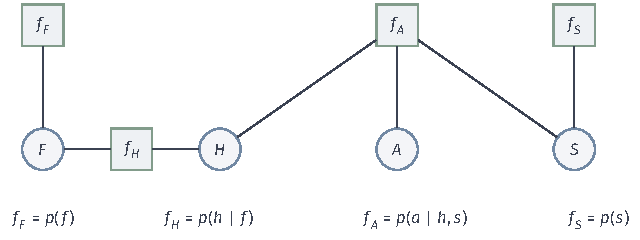
\includegraphics[width=108.433mm]{figures/06-probabilistic-graphical-models/01-representation/tikz/pgm-representations-alarm-factor-graph/figure.pdf}
  \caption{报警模型的四因子表示。圆形表示随机变量，方形表示局部条件分布或先验函数；$f_H$使用$F,H$，$f_A$使用$H,A,S$，连线记录函数的输入变量。}
  \label{fig:pgm-representations-alarm-factor-graph}
\end{figure}

Markov网络的每个势也对应一个因子节点，连接所有作用域变量。边势和一元势可以各自保留为小因子，无需预先合成极大团表。将每个因子的输入变量两两连接，又可得到无向变量图；该图记录共同作用域，但不再区分它由多少个局部函数组成。

三个二元势相乘的$g=\psi_{\{1,2\}}\psi_{\{2,3\}}\psi_{\{1,3\}}$生成一个无向三角形，一般三元势$\psi_{\{1,2,3\}}$也对应同一个团。前者明确分为三个二元函数，后者可能包含不可约的三元作用。三角形本身没有条件独立性来区分两种表示，因子图却显示了局部函数的数量和阶数。这些额外信息来自输入函数的分解。

\subsection{表示的非唯一性}
\label{sec:pgm-representations-nonuniqueness}

合并局部函数会改变因子图，而整个函数可以保持原样。图~\ref{fig:pgm-representations-factor-grouping}将三个二元因子相乘为一个三元因子，六边环随之变成星形。星形虽无环，中心表却从单个二元因子的$r^2$项变为$r^3$项。计算开销因此需要同时看连接结构与因子大小。

\begin{figure}[htbp]
  \centering
  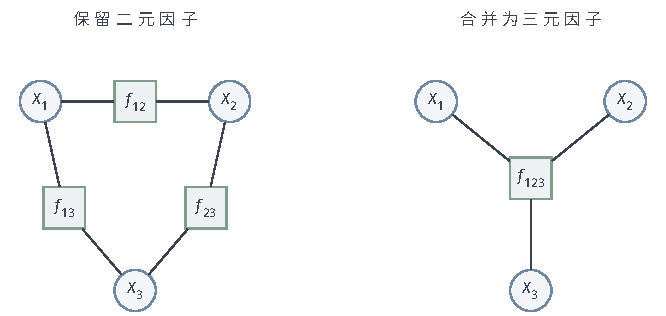
\includegraphics[width=112.000mm]{figures/06-probabilistic-graphical-models/01-representation/tikz/pgm-representations-factor-grouping/figure.pdf}
  \caption{合并因子前后的同一联合函数。左图由三个二元因子构成环，右图以$f_{123}=f_{12}f_{23}f_{13}$形成一个三元因子的星形。两种因子图都生成三角形变量图，局部表规模与连接结构不同。}
  \label{fig:pgm-representations-factor-grouping}
\end{figure}

函数相乘可以合并，能否拆分则要看函数值。若二元函数可以写成两个一元函数的乘积，即满足
\[
  f_{12}(x_1,x_2)=u(x_1)v(x_2),
\]
它的离散函数表就是外积，秩至多为$1$。式~\eqref{eq:pgm-representations-cycle-potentials}的表$\left(\begin{smallmatrix}2&1\\1&2\end{smallmatrix}\right)$行列式为$3$，无法写成两个一元函数的乘积。三元势拆成三个二元势时，同样需要核验具体函数是否具有相应结构。

共享变量还允许在两个因子间转移权重，同时保持总乘积。这种\term{重新参数化}（reparameterization）可以保留原作用域。例如用严格正的$h(x_2)$定义
\[
  \widetilde f_{12}=f_{12}h(x_2),\qquad
  \widetilde f_{23}=\frac{f_{23}}{h(x_2)}.
\]
两新因子的$h$恰好约去，总乘积与原来相同。若仅将一个因子乘以正常数，未归一化函数$g$便同比缩放，调整$Z$后仍得到同一分布$p$。前一种变换保留联合函数，后一种保留归一化分布，二者的代数要求不同。

变量节点的删除也能从因子图读出一些独立性。设$A,B,S\subseteq V$两两不交，$A,B$非空。对非负概率因子分解，删除\emph{变量节点}$S$后，若$A$与$B$分处不同连通分量，给定$\bm{X}_S=\bm{s}$便可按分量整理乘积，并分别归一化，得到$\bm{X}_A\perp\bm{X}_B\mid\bm{X}_S$。运算使用条件分布有效的$\bm{s}$；有限离散情形要求$p(\bm{X}_S=\bm{s})>0$。该分离提供充分保证，具体函数还可能隐含其他独立性。

报警因子图一直有连接$H-f_A-S$，函数却满足$\sum_a f_A(h,a,s)=1$，消去报警后，两原因仍然边缘独立。这条条件归一化等式保留在函数内，拓扑没有显示它。因子图适合据作用域安排计算；碰撞关系仍需原有向图的条件语义，无向Markov约束则由相应变量图的分离判断。

\subsection{因子图上的局部计算}
\label{sec:pgm-representations-local-computation}

有了因子图，就可以在它上面组织推断计算了。本章只说明最基本的局部操作如何由图的连接决定，具体的消元顺序选择、复杂度分析和消息复用留给第~\ref{chap:pgm-elimination}章与第~\ref{chap:pgm-junction-tree}章。先从最常见的问题说起：观测到一部分变量后，想求另一部分（查询）变量的后验分布，就要把既未观测、也不查询的变量全部求和消去。下面的局部计算采用有限离散取值变量和有限个非负实值因子，乘积可以归一化为合法分布。所给证据满足$p(\bm X_S=\bm s)>0$。这些条件保证下面的求和都是有限和，后验归一化分母为正，有限候选集上的最大值也能取得。一般函数的因子图定义本身不要求变量离散；连续查询还需另行处理积分、条件密度版本以及最大值是否取得，不能仅靠下述有限运算公式得到这些保证。

观测$\bm{X}_S=\bm{s}$后，将相关因子中的证据坐标固定在该值。以$Q\subseteq V\setminus S$为查询集，其他待消变量组成$R=V\setminus(Q\cup S)$。将它们求和消去，得到查询的未归一化边缘函数：
\begin{equation}
  \widetilde p(\bm{x}_Q,\bm{s})
  =\sum_{\bm{x}_R}
  \prod_{\alpha\in\mathcal{F}}
  f_\alpha(\bm{x}_{D_\alpha\setminus S},\bm{s}_{D_\alpha\cap S}).
  \label{eq:pgm-representations-marginal-query}
\end{equation}
若$p(\bm{s})>0$，对$\bm{x}_Q$求和得到的常数可将$\widetilde p$归一化，得到后验边缘分布。

分配律使每步计算可以只处理相关因子：$u$不含$x_i$时，有$\sum_{x_i}u\,v=u\sum_{x_i}v$。因此，收集与$x_i$相连的因子，相乘再求和，将所得新函数接到剩余作用域即可。式~\eqref{eq:pgm-representations-cycle-message}就是将两个边因子经消元变为$\{1,3\}$上的新因子。连接关系由此给出每步的输入函数及输出变量集。

求后验边缘回答的是“各状态分别有多可能”，但很多实际问题要的不是概率，而是“最可能的完整情形是什么”：如图像分割中要给出一整幅最可能的标签配置，故障诊断中要给出一组最可能的状态。这时汇总未知变量的算子要从“求和”换成“取最大值”。寻找全部非证据变量的最可能联合配置时，改对其完整配置取最大值：
\[
  \max_{\bm{x}_{V\setminus S}}
  \prod_{\alpha\in\mathcal{F}}f_\alpha.
\]
该查询称为\term{最可能解释}（most probable explanation, MPE）。$Z$对所有候选配置相同，最大化未归一化权重就能比较候选；每步记录取得最大值的状态，结束后回溯，才能恢复最优配置。若仅对部分变量求最优，其他未观测变量需先求和，则形成\term{边缘最大后验推断}（marginal maximum a posteriori inference, marginal MAP）问题。沿用查询集$Q$与其余待消集$R$，它寻找的是
\begin{equation}
  \bm x_Q^\star\in
  \argmax_{\bm x_Q}\left\{
    \sum_{\bm x_R}
    \prod_{\alpha\in\mathcal F}
      f_\alpha(\bm x_{D_\alpha\setminus S},
        \bm s_{D_\alpha\cap S})
  \right\}.
  \label{eq:pgm-representations-marginal-map}
\end{equation}
内层求和汇总没有被选作优化目标的变量，外层最大化再选择查询配置；证据的归一化常数不随$\bm x_Q$改变，所以不影响这个选择。边缘概率查询输出每个查询配置的后验概率，MPE输出全部非证据变量的最优联合配置，边缘MAP则输出查询变量的最优配置。这三个任务保留和消去的信息不同。

边缘MAP混合求和与最大化，两种算子的先后次序会影响结果。用一个人工构造的严格正二元概率表即可看出差别：以$x=0,1$为行、$y=0,1$为列，取
\[
  \bigl[p(x,y)\bigr]=
  \begin{pmatrix}
    0.36&0.04\\
    0.30&0.30
  \end{pmatrix}.
\]
四项之和为$1$，MPE选择最大单格$(x,y)=(0,0)$，概率为$0.36$。若只希望选择$x$，两行的边缘概率分别是$0.40$与$0.60$，边缘MAP便选择$x=1$。先求和再取最大值得到$\max_x\sum_y p(x,y)=0.60$；若颠倒次序，两列最大值相加却得到$\sum_y\max_x p(x,y)=0.36+0.30=0.66$。后一个计算允许第一列选$x=0$、第二列选$x=1$，不再要求同一个$x$配置解释全部$y$状态，因此改变了原查询。

一般混合查询不能任意交换这两个算子，但作用域相互分开时可能提前处理某个最大化。例如固定其余变量$\bm z$后，若乘积为$h(x,\bm z)u(y,\bm z)$，非负性使
\[
  \max_x\sum_y h(x,\bm z)u(y,\bm z)
    =\bigl[\max_x h(x,\bm z)\bigr]
      \bigl[\sum_y u(y,\bm z)\bigr].
\]
这里$h$不含$y$、$u$不含$x$，所以$x$的最佳选择不随被汇总的$y$改变。是否合法换序，要检查当前相关因子的作用域；一个通用的正确顺序是先消去全部$R$，再最大化$Q$，具体图结构可能允许更多安排。

边缘概率查询和完整配置MPE都用乘法组合函数，区别在于汇总状态的算子：\term{和积}（sum-product）随后求和，\term{最大积}（max-product）随后取最大值。在四环的式~\eqref{eq:pgm-representations-cycle-message}中，将求和换为最大化，两端相同时得到$4$，不同时得到$2$；原来的求和结果则为$5$和$4$。输入因子相同，消元算子决定了当前函数回答的是概率汇总还是最优权重。边缘MAP同时使用两种汇总，仍需保留刚才说明的顺序约束。

和积与最大积两套计算的步骤几乎完全相同：都是收集相邻因子加以组合，再对待消变量的取值做汇总，唯一区别是组合用乘法、汇总分别用求和或取最大值。既然流程相同，可将其抽象成一种统一形式，使同一套消息传递实现只需替换两个运算就能服务不同查询；这种抽象还能说明“合法重组”依赖哪些代数性质。将组合函数与汇总状态两项操作抽象出来，就得到\term{半环}（semiring）形式：以$\otimes$组合局部函数，以$\oplus$汇总待消变量的不同取值。采用交换半环时，两运算都满足结合律、交换律，$\otimes$对$\oplus$还满足分配律。以$e_\oplus$记$\oplus$的单位元、$e_\otimes$记$\otimes$的单位元，并有吸收关系$a\otimes e_\oplus=e_\oplus$。这组运算条件让收集因子后的消元写成
\begin{equation}
  \begin{aligned}
    h(\bm{x}_{D\setminus\{i\}})
    &=
    \bigoplus_{x_i}
    \ \bigotimes_{\alpha:\,i\in D_\alpha}
    f_\alpha(\bm{x}_{D_\alpha}),\\
    D&=\bigcup_{\alpha:\,i\in D_\alpha}D_\alpha.
  \end{aligned}
  \label{eq:pgm-representations-semiring-elimination}
\end{equation}
在非负实数上，$(\oplus,\otimes)=(+,\times)$就是和积，其$(e_\oplus,e_\otimes)=(0,1)$；最大积用$(\max,\times)$，单位元也为$0$和$1$。取对数后，在$\mathbb{R}\cup\{-\infty\}$上使用$(\max,+)$，有$(e_\oplus,e_\otimes)=(-\infty,0)$，零权重变为$-\infty$。每种运算都具备上述分配关系，所以同样的收集因子、局部消元步骤可以用于相应的纯和积或纯最大积查询\scite{pgm-overview-kschischang2001}。这里每次汇总只有有限项，普通半环的公理已足以支持重组；若要进行无穷汇总或连续积分，还需相应的收敛与交换运算条件。一个固定的交换半环也不会自动消除边缘MAP混用求和与最大化的顺序限制。

一次消元留下剩余变量上的函数，它概括了被消变量对后续计算的影响。沿图传递这样的函数，就是消息传递的基本操作。在无环因子图上，移除一条边将计算分成不重叠的两部分，一侧的消息能汇总该侧全部影响，因而和积可精确求边缘。有环图反复更新消息时，传回的信息可能已包含先前从当前节点发出的影响，两侧不再分离；后文的环置信传播将讨论这一问题。另一种精确组织是先按顺序消元形成大团，再在团之间安排消息。第~\ref{chap:pgm-elimination}章讨论消元顺序与复杂度，第~\ref{chap:pgm-junction-tree}章介绍消息的组织及复用。

\section{本章小结}
\label{sec:pgm-representations-summary}

图转换会同时涉及分布值、独立性声明和计算结构，三者需分别比较。I-map要求图声明属于分布的真实独立性，即$\mathcal{I}(\mathcal{G})\subseteq\mathcal{I}(p)$，D-map方向相反。当前查询的祖先道德图精确复现d-分离，整图道德化通常减少可见的独立性。碰撞结构与无弦四环分别展示两类图完美表示的边界；弦图与父集成团的有向图则可互相保留全部图分离关系。

祖先道德图将查询两侧的因子分开归一化，从而证明d-分离的可靠性。对未分离查询，离散条件表与线性高斯参数的非平凡多项式提供相容分布中的依赖见证，给出这两个模型类的完备性。若一个固定分布的全部独立性都要对应图的d-分离，还需忠实性，将模型类的存在保证加强到该分布的完美映射。

局部函数的重组可以保留完整分布：有向条件因子成为道德图的团势，弦图团势沿完美消元序生成条件表，非弦图则借填充边容纳中间函数。四环的数值计算中，新增边让图少声明一项独立性，原函数却继续满足它。只有允许新条件表各自自由变化，转换后的完整图模型族才更大。

因子图用变量与函数的连接保留输入分解，按查询选择求和或最大化，实现局部组合与消元。同一分布有多种因子图，连接方式和局部函数的阶数共同决定开销。给定因子和查询后，接下来的任务是选择消元顺序，控制中间函数的大小，并复用已完成的局部计算。

\paragraph{扩展阅读}
Koller与Friedman的教材系统比较有向、无向及因子化表示。书中的转换例子可结合本章的三项比较继续阅读：哪些联合概率保持原样，哪些独立性仍由新图保证，以及局部函数的重组怎样影响推断所需的中间表\scite{pgm-koller2009}。
